\subsection{RQ2: Trust under Missing, Forged and Imperfect Evidence}
\label{sec:ev-rq2}

RQ2 asks whether provenance-sound eligibility (P) keeps unsafe tools away from the model when metadata is
missing, forged or verified imperfectly, and what this costs in utility. Proposition~1 guarantees soundness only
if safety-relevant evidence is truthful (formal); the experiments below measure how exposure behaves when that
assumption is relaxed (simulated), whether the result depends on how the reference labels were built
(labelled), and whether the labels agree with what real servers do when executed (observed).

\emph{Protocol.} A read-only policy is applied to the 394 requests of the single-tool test sample and the
development split; Exp@5 is the share of the 273 requests with read-only gold tools whose top five contain a
tool that is not read-only under $J_B$, and Util@5 the share whose top five contain a gold tool. Each encoding of
the policy is applied to \pamcp{}'s retrieval stage and to MCP-Zero. Forgery is simulated by letting a share
$\delta$ of the servers declare \texttt{readOnlyHint=true} on every tool and launder their descriptions (five
seeds per $\delta$); the verifier is simulated with false-accept rate $\varphi$, false-reject rate $\psi$ and
probe coverage $\kappa$. For the observed comparison, the six MCP reference servers of the registry were started
from their published packages (current versions) in a sandbox; each of their 37 registry tools was called once
with schema-derived arguments under system-call tracing and file-system snapshots, and a state change was
recorded when the call wrote, renamed or deleted user files, the server's store or version-control content.

\begin{table}[t]
\centering
\caption{Encodings of a read-only policy over 273 requests with read-only gold tools: eligible share of the
registry, unsafe tools admitted (of 120, $J_B$), exposure and utility of the top five for \pamcp{}'s retrieval
stage and MCP-Zero, and exposure when 20\% of the servers forge and launder their metadata (verifier
false-accept rate 5\%, mean of five seeds).}
\label{tab:ev-encodings}
\scriptsize
\setlength{\tabcolsep}{2.2pt}
\begin{tabular}{@{}lrrrrrrr@{}}
\toprule
 & & & \multicolumn{2}{c}{\pamcp{} retr.} & \multicolumn{2}{c}{MCP-Zero} & $\delta{=}0.2$ \\
\cmidrule(lr){4-5}\cmidrule(lr){6-7}\cmidrule(l){8-8}
Encoding & Elig. & Unsafe & Exp@5 & Util@5 & Exp@5 & Util@5 & Exp@5 \\
\midrule
no filter & 100.0 & 120 & 42.5 & 49.8 & 26.4 & 76.6 & 43.7 \\
MCP default (display only) & 100.0 & 120 & 42.5 & 49.8 & 26.4 & 76.6 & 43.7 \\
closed-world annotations & 7.7 & 1 & 31.5 & 0.4 & 0.0 & 0.4 & 58.7 \\
lexical cues & 67.8 & 21 & 9.9 & 41.0 & 12.5 & 65.6 & 8.8 \\
verified evidence (P) & 77.0 & 0 & 0.0 & 46.2 & 0.0 & 72.2 & 5.5 \\
observed + lexical fallback & 77.0 & 0 & 0.0 & 46.2 & 0.0 & 72.2 & 5.5 \\
attested only & 26.4 & 0 & 0.0 & 16.5 & 0.0 & 18.3 & 5.8 \\
\bottomrule
\end{tabular}
\end{table}


\emph{Declared metadata is not evidence.} Table~\ref{tab:ev-encodings} compares the encodings at full
verification coverage. Without a filter, and under MCP's default of displaying annotations without enforcing
them, 42.5\% of the requests receive an unsafe tool among \pamcp{}'s top five (26.4\% for MCP-Zero). Treating
the annotations as a closed world keeps only the 44 annotated tools; the one unsafe tool among them then reaches
31.5\% of the lists while utility collapses to 0.4\%. Lexical cues admit 21 of the 120 unsafe tools (Exp@5 9.9\%,
Util@5 41.0\%; they flag 82.5\% of the unsafe tools at a precision of 0.54). Verified evidence admits none, keeps
77.0\% of the registry eligible and costs 3.6 points of utility for \pamcp{}'s retrieval (46.2\% against 49.8\%)
and 4.4 points for MCP-Zero (72.2\% against 76.6\%); with lower probe coverage, exposure stays at zero and utility
follows the eligible share (Fig.~\ref{fig:ev-exposure}a).

\begin{figure*}[t]
\centering
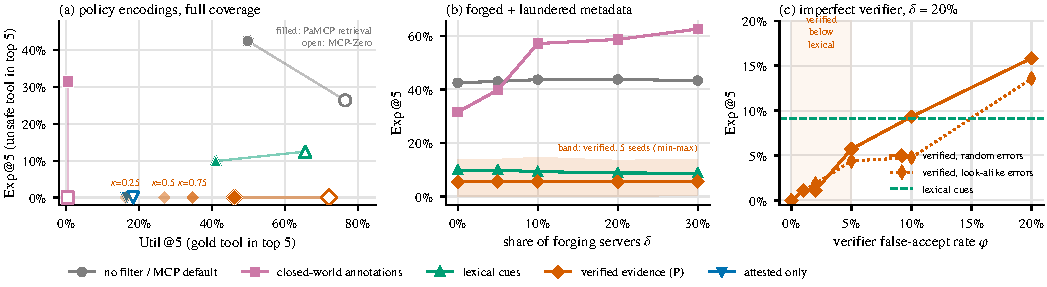
\includegraphics[width=\textwidth]{fig_rq2_exposure}
\caption{Exposure under a read-only policy (273 requests). (a) Exposure against utility per encoding at full
coverage, and verified evidence at lower probe coverage $\kappa$. (b) Exposure as a share $\delta$ of servers
forges annotations and launders descriptions (verifier false-accept rate 5\%; mean of five seeds, band: range of
the seeds for verified evidence). (c) Exposure of verified evidence against the false-accept rate, with errors at
random or on look-alike unsafe tools, against the lexical encoding.}
\label{fig:ev-exposure}
\end{figure*}

\emph{Forged and imperfect evidence.} Forgery breaks the closed-world reading: its exposure rises from 31.5\% to
57.1\% when a tenth of the servers forge and to 62.6\% at 30\% (Fig.~\ref{fig:ev-exposure}b). Laundered
descriptions barely affect lexical cues (8.7--9.9\%), because tool names carry most cues. Verified evidence is
independent of $\delta$ by construction of the probe: with a 5\% false-accept rate its exposure is 5.4--5.6\%
at every $\delta$, including $\delta=0$ (five seeds each), at a utility of 46.1--46.7\%; which unsafe tools are
falsely accepted varies with the seed (0.0--14.7\% per seed). Exposure grows roughly linearly with the
false-accept rate (1.1\%, 5.7\%, 9.3\% and 15.8\% at $\varphi$ of 1, 5, 10 and 20\%; Fig.~\ref{fig:ev-exposure}c);
errors concentrated on look-alike unsafe tools are not worse. Verified evidence stays below the lexical encoding
(9.2\%) up to $\varphi=5\%$ with random errors and up to 10\% with look-alike errors: a verifier must be at least
this accurate to help. False rejections cost utility instead ($\psi=0.2$: 46.2\% to 39.1\%).

\begin{figure}[t]
\centering
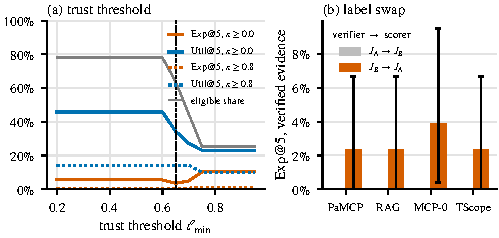
\includegraphics[width=\columnwidth]{fig_rq2_trust}
\caption{(a) Exposure, utility and eligible share against the trust threshold $\ell_{\min}$ ($\delta=0.2$,
$\varphi=5\%$), with and without a minimum probe coverage $\kappa\ge0.8$. (b) Exposure of verified evidence when
the verifier is simulated from one labelling and scored on the other (cluster-bootstrap 95\% CI).}
\label{fig:ev-trust}
\end{figure}

\emph{Trust threshold.} Raising $\ell_{\min}$ from 0.55 to 0.65, the level of observed evidence, lowers exposure
from 5.5\% to 3.5\% and utility from 45.8\% to 34.4\%; requiring $\kappa\ge0.8$ as well lowers them to 0.6\% and
14.3\% (Fig.~\ref{fig:ev-trust}a). Above 0.75 only attested evidence qualifies and exposure rises again to
10.3\%, because the few falsely accepted attested tools reach many lists of a pool of 25.4\% of the registry. A
stricter threshold therefore does not lower exposure by itself; exposure must be read with the eligible pool.

\emph{Independence of the reference labels.} With the verifier simulated from $J_A$ and scoring on $J_B$, zero
exposure at $\varphi=0$ is guaranteed by the inclusion of the unsafe sets and carries no empirical content.
Swapping the roles removes the inclusion: a verifier simulated from $J_B$ admits the 11 tools that only $J_A$
considers unsafe, and verified evidence then exposes 2.3\% of the requests for \pamcp{}'s retrieval, RAG-MCP and
ToolScope and 3.9\% for MCP-Zero (Fig.~\ref{fig:ev-trust}b), against 9.9\% for lexical cues under the original
scoring. The protection therefore survives a disagreement between independent labellers, at a non-zero rate that
measures their disagreement rather than the verifier.

\begin{table}[t]
\centering
\caption{State changes observed when executing the 30 exercised tools of six MCP
reference servers, against the two labellings and the servers' current annotations. FS: labelled read-only but
observed to modify state (false safe; Wilson 95\% CI); Unconf.: labelled state-changing, not triggered by the
probe.}
\label{tab:ev-observed}
\scriptsize
\setlength{\tabcolsep}{3pt}
\begin{tabular}{@{}lrrrrrr@{}}
\toprule
Reference & TP & FS & Unconf. & TN & False-safe rate (\%) & Agree. \\
\midrule
$J_A$ (Sonnet) & 13 & 0 & 0 & 17 & 0 [0, 22.8] & 100 \\
$J_B$ (Opus) & 13 & 0 & 0 & 17 & 0 [0, 22.8] & 100 \\
live annotations & 13 & 0 & 5 & 12 & 0 [0, 22.8] & 83 \\
\bottomrule
\end{tabular}
\end{table}


\begin{figure*}[t]
\centering
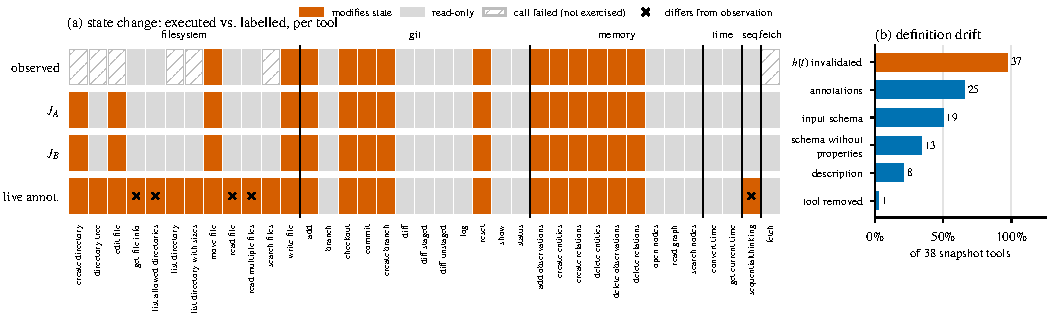
\includegraphics[width=\textwidth]{fig_rq2_observed}
\caption{Executed reference servers. (a) Per registry tool: state change observed under tracing, the two
labellings and the servers' current annotations (not read-only unless \texttt{readOnlyHint=true}). (b) Changes of
the live definitions against the registry snapshot; every changed definition changes $h(t)$.}
\label{fig:ev-observed}
\end{figure*}

\emph{Observed effects of executed servers.} All six reference servers started; 30 of the 37 probed tools
completed their call (six file-system calls received arguments the synthesiser could not make valid, e.g.\ an
edit whose target text is absent, and the fetch call was blocked by the sandbox's network policy), and 13 of them changed state: the memory server's six writers rewrite its store, five
Git tools commit, stage, reset, branch or check out, and two file-system tools write or move files
(Fig.~\ref{fig:ev-observed}a). Both labellings agree with every exercised call (Table~\ref{tab:ev-observed}):
no tool observed to change state is labelled read-only (0 of 13; Wilson upper bound 22.8\%), and no label of a
state change went unconfirmed. The servers now publish annotations for 25 of these tools, none in the registry
snapshot; none claims read-only for an observed state change, and they are conservative on 5 read-only tools.
Since the snapshot, every one of the 37 surviving definitions has changed (annotations 25, input schemas 19,
descriptions 8; Fig.~\ref{fig:ev-observed}b), one tool was removed and five were added; 13 file-system tools now
publish input schemas without properties, which the official Python SDK rejects. Bound to $h(t)$, every piece of
evidence about these servers would have been invalidated and re-established before use.

\emph{Interpretation.} Provenance-sound eligibility removes the exposure that declared or lexical metadata
leaves (9.9--42.5\%) at a utility cost of 3.6--4.4 points, and degrades gracefully, roughly in proportion to the
verifier's false-accept rate, when evidence is imperfect. The zero exposure of an error-free verifier is a
property of the simulation; the swapped labels bound the effect of labeller disagreement at 2.3--3.9\%, and
execution confirms the labels on the state changes of 30 reference tools. These servers are maintained by the
protocol's authors and are not adversarial; behaviour against malicious third-party servers is outside the
observed evidence (Section~\ref{sec:ev-threats}). The drift measurement supports binding evidence to $h(t)$:
in the ecosystem studied, definitions change often enough that unbound evidence would be stale.
